\chapter{Linked Lists}

In this chapter, we continue to study implementations of the \mbox{\texttt{List}}
interface, this time using pointer-based data structures rather than
arrays.  The structures in this chapter are made up of nodes that
contain the list items.  The nodes are linked together into a sequence
using references (pointers).  We first study singly-linked lists, which
can implement \mbox{\texttt{Stack}} and (FIFO) \mbox{\texttt{Queue}} operations in constant time
per operation.

Compared to array-based list implementations, linked lists have their
advantages and disadvantages.  The primary disadvantage is that we
lose the ability to access any element using \mbox{\texttt{get({\color{var}i})}} or \mbox{\texttt{set({\color{var}i},{\color{var}x})}} in
constant time.  Instead, we have to walk through the list, one element
at a time, until we reach the \mbox{\texttt{{\color{var}i}}}th element.  The primary advantage is
that they are more dynamic:  Given a reference to any list node \mbox{\texttt{{\color{var}u}}}, we
can delete \mbox{\texttt{{\color{var}u}}} or insert a node adjacent to to \mbox{\texttt{{\color{var}u}}} in constant time. This
is true no matter where \mbox{\texttt{{\color{var}u}}} is in the list.


\section{\mbox{\texttt{SLList}}: A Singly-Linked List}
\seclabel{sllist}

An \mbox{\texttt{SLList}} (singly-linked list) is a sequence of \mbox{\texttt{Node}}s.  Each node
\mbox{\texttt{{\color{var}u}}} stores a data value \mbox{\texttt{{\color{var}u}.{\color{var}x}}} and a reference \mbox{\texttt{{\color{var}u}.{\color{var}next}}} to the next node in
the sequence.  For the last node \mbox{\texttt{{\color{var}w}}} in the sequence, $\mbox{\texttt{{\color{var}w}.{\color{var}next}}} = \mbox{\texttt{{\color{var}null}}}$

% TODO: Remove constructors from SLList.Node
\begin{Verbatim}[tabsize=2,frame=single,commandchars=\\@\$,label=\texttt{SLList},labelposition=topline]
	@\color@keyword$class$ Node {
		@\color@keyword$T$ @\color@var$x$;
		Node @\color@var$next$;
	}
\end{Verbatim}

For efficiency, an \mbox{\texttt{SLList}} uses variables \mbox{\texttt{{\color{var}head}}} and \mbox{\texttt{{\color{var}tail}}} to keep
track of the first and last node in the sequence, as well as an integer
\mbox{\texttt{{\color{var}n}}} to keep track of the length of the sequence:
\begin{Verbatim}[tabsize=2,frame=single,commandchars=\\@\$,label=\texttt{SLList},labelposition=topline]
	Node @\color@var$head$;
	Node @\color@var$tail$;
	@\color@keyword$int$ @\color@var$n$;
\end{Verbatim}
A sequence of \mbox{\texttt{Stack}} and \mbox{\texttt{Queue}} operations is illustrated on an
\figref{sllist} in \figref{sllist}.

\begin{figure}
  \begin{center}
    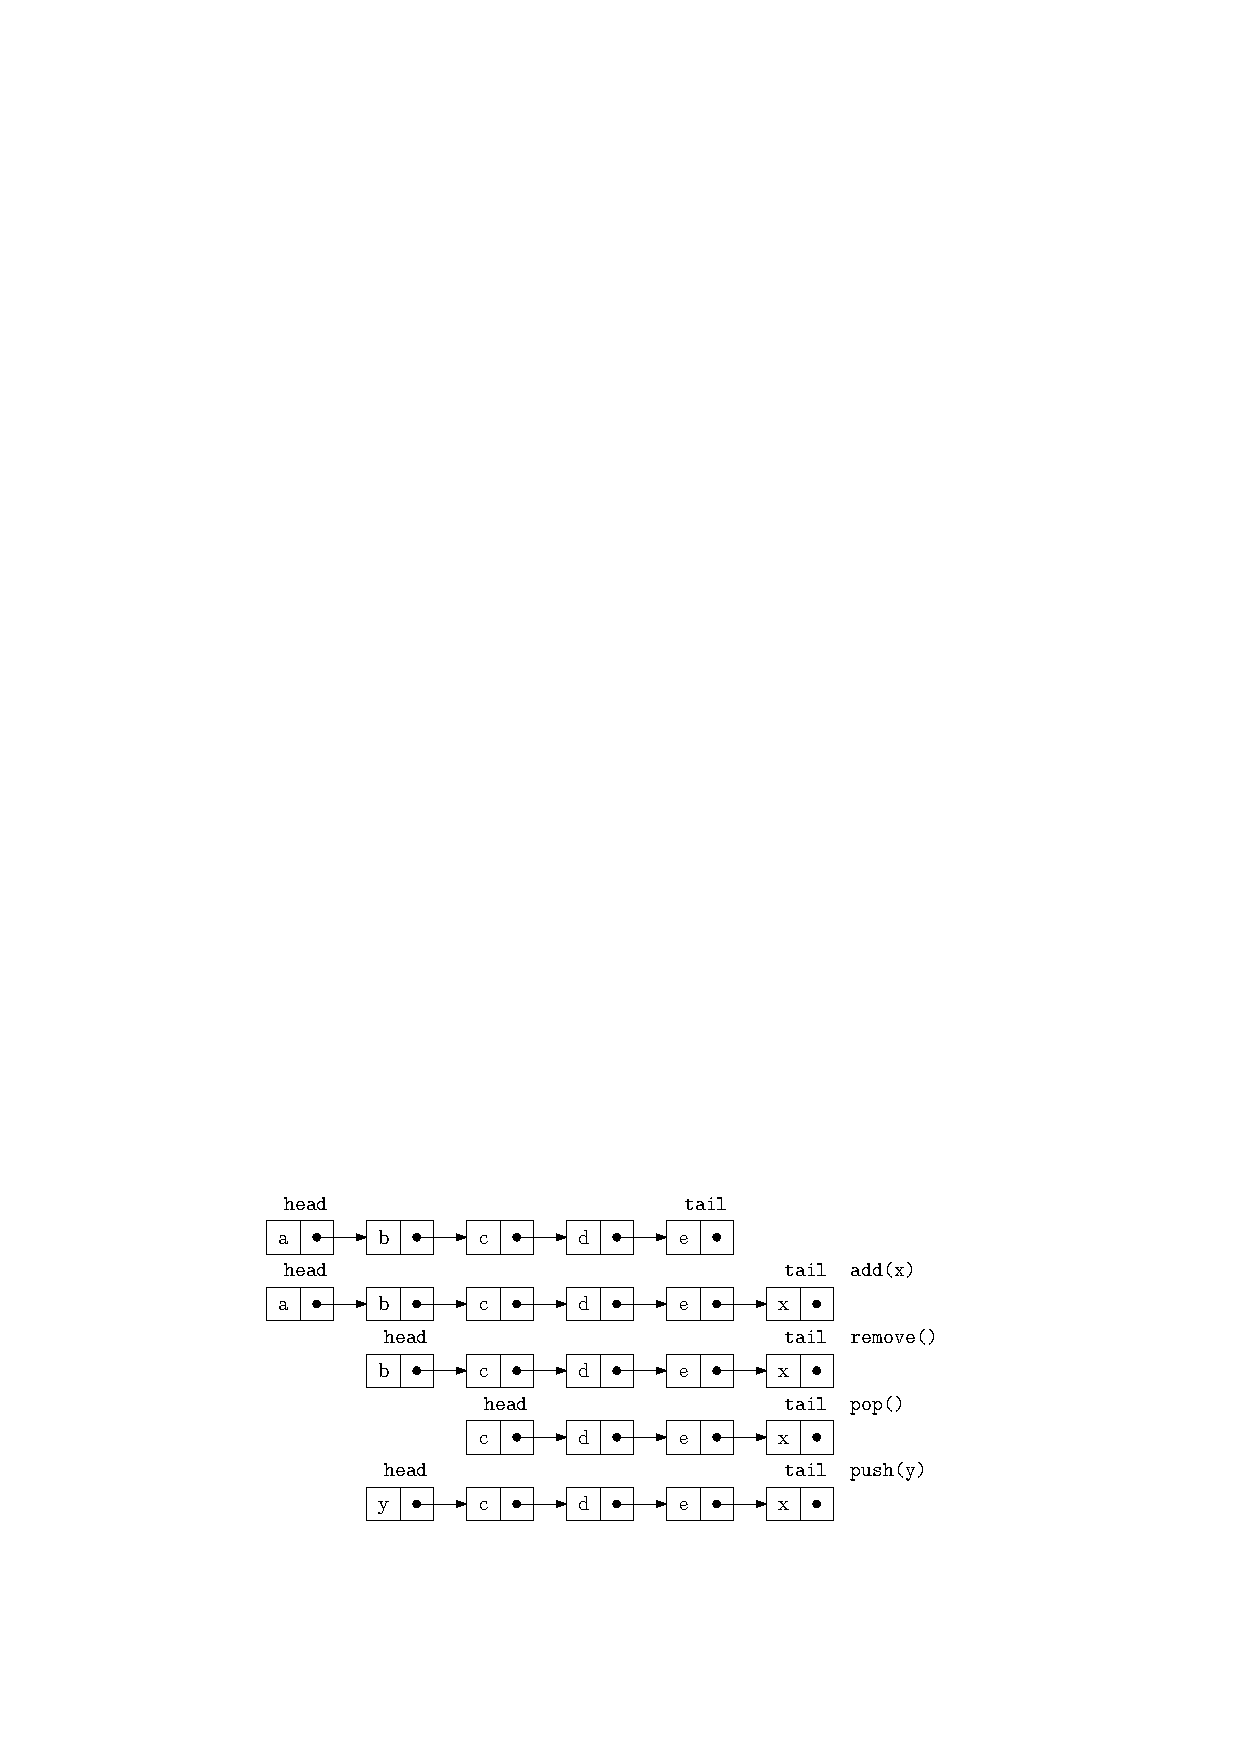
\includegraphics{figs/sllist}
  \end{center}
  \caption{A sequence of \mbox{\texttt{Queue}} (\mbox{\texttt{add({\color{var}x})}} and \mbox{\texttt{remove()}}) and \mbox{\texttt{Stack}} (\mbox{\texttt{push({\color{var}x})}} and \mbox{\texttt{pop()}}) operations in an \mbox{\texttt{SLList}}.}
  \figlabel{sllist}
\end{figure}


An \mbox{\texttt{SLList}} can efficiently implement the \mbox{\texttt{Stack}} operations \mbox{\texttt{push()}}
and \mbox{\texttt{pop()}} by adding and removing elements at the head of the sequence.
The \mbox{\texttt{push()}} operation simply creates a new node \mbox{\texttt{{\color{var}u}}} with data value \mbox{\texttt{{\color{var}x}}},
sets \mbox{\texttt{{\color{var}u}.{\color{var}next}}} to the old head of the list and makes \mbox{\texttt{{\color{var}u}}} the new head
of the list. Finally, it increments \mbox{\texttt{{\color{var}n}}} since the size of the \mbox{\texttt{SLList}}
has increased by one:

\begin{Verbatim}[tabsize=2,frame=single,commandchars=\\@\$,label=\texttt{SLList},labelposition=topline]
	@\color@keyword$T$ push(@\color@keyword$T$ @\color@var$x$) {
		Node @\color@var$u$ = @\color@keyword$new$ Node();
		@\color@var$u$.@\color@var$x$ = @\color@var$x$;
		@\color@var$u$.@\color@var$next$ = @\color@var$head$;;
		@\color@var$head$ = @\color@var$u$;
		@\color@keyword$if$ (@\color@var$n$ == 0)
			@\color@var$tail$ = @\color@var$u$;
		@\color@var$n$++;
		@\color@var$return$ @\color@var$x$;
	}
\end{Verbatim}

The \mbox{\texttt{pop()}} operation, after checking that the \mbox{\texttt{SLList}} is not empty,
removes the head by setting $\mbox{\texttt{{\color{var}head}}}=\mbox{\texttt{{\color{var}head}.{\color{var}next}}}$ and decrementing \mbox{\texttt{{\color{var}n}}}.
A special case occurs when the last element is being removed, in which case \mbox{\texttt{{\color{var}tail}}} is set to \mbox{\texttt{{\color{var}null}}}:

\begin{Verbatim}[tabsize=2,frame=single,commandchars=\\@\$,label=\texttt{SLList},labelposition=topline]
	@\color@keyword$T$ pop() {
		@\color@keyword$if$ (@\color@var$n$ == 0)	@\color@var$return$ @\color@var$null$;
		@\color@keyword$T$ @\color@var$x$ = @\color@var$head$.@\color@var$x$;
		@\color@var$head$ = @\color@var$head$.@\color@var$next$;
		@\color@keyword$if$ (--@\color@var$n$ == 0) @\color@var$tail$ = @\color@var$null$;
		@\color@var$return$ @\color@var$x$;
	}	
\end{Verbatim}

Clearly both the \mbox{\texttt{push({\color{var}x})}} and \mbox{\texttt{pop()}} operations run in $O(1)$ time.

\subsection{Queue Operations}

An \mbox{\texttt{SLList}} can also efficiently implement the FIFO queue operations \mbox{\texttt{add({\color{var}x})}} and \mbox{\texttt{remove()}}.  Removals are done from the head of the list, and are identical to the \mbox{\texttt{pop()}} operation:

\begin{Verbatim}[tabsize=2,frame=single,commandchars=\\@\$,label=\texttt{SLList},labelposition=topline]
	@\color@keyword$T$ remove() {
		@\color@keyword$if$ (@\color@var$n$ == 0)	@\color@var$return$ @\color@var$null$;
		@\color@keyword$T$ @\color@var$x$ = @\color@var$head$.@\color@var$x$;
		@\color@var$head$ = @\color@var$head$.@\color@var$next$;
		@\color@keyword$if$ (--@\color@var$n$ == 0) @\color@var$tail$ = @\color@var$null$;
		@\color@var$return$ @\color@var$x$;
	}	
\end{Verbatim}

Additions, on the other hand, are done at the tail of the list.  In most
cases, this is done by setting $\mbox{\texttt{{\color{var}tail}.{\color{var}next}}}=\mbox{\texttt{{\color{var}u}}}$, where \mbox{\texttt{{\color{var}u}}} is the newly
created node that contains \mbox{\texttt{{\color{var}x}}}.  However, a special case occurs when
$\mbox{\texttt{{\color{var}n}}}=0$, in which case $\mbox{\texttt{{\color{var}tail}}}=\mbox{\texttt{{\color{var}head}}}=\mbox{\texttt{{\color{var}null}}}$.  In this case, both \mbox{\texttt{{\color{var}tail}}}
and \mbox{\texttt{{\color{var}head}}} are set to \mbox{\texttt{{\color{var}u}}}.

\begin{Verbatim}[tabsize=2,frame=single,commandchars=\\@\$,label=\texttt{SLList},labelposition=topline]
	@\color@var$boolean$ add(@\color@keyword$T$ @\color@var$x$) {
		Node @\color@var$u$ = @\color@keyword$new$ Node();
		@\color@var$u$.@\color@var$x$ = @\color@var$x$;
		@\color@keyword$if$ (@\color@var$n$ == 0) {
			@\color@var$head$ = @\color@var$u$;
		} @\color@keyword$else$ {
			@\color@var$tail$.@\color@var$next$ = @\color@var$u$;
		}
		@\color@var$tail$ = @\color@var$u$;
		@\color@var$n$++;
		@\color@var$return$ @\color@var$true$;
	}
\end{Verbatim}

Clearly, both \mbox{\texttt{add({\color{var}x})}} and \mbox{\texttt{remove()}} take constant time.

\subsection{Summary}

The following theorem summarizes the performance of an \mbox{\texttt{SLList}}:

\begin{thm}\thmlabel{sllist}
  An \mbox{\texttt{SLList}} implements the \mbox{\texttt{Stack}} and (FIFO) \mbox{\texttt{Queue}} interfaces.  
  The \mbox{\texttt{push({\color{var}x})}}, \mbox{\texttt{pop()}}, \mbox{\texttt{add({\color{var}x})}} and \mbox{\texttt{remove()}} operations run
  in $O(1)$ time per operation.
\end{thm}

An \mbox{\texttt{SLList}} comes very close to implementing the full set of \mbox{\texttt{Deque}}
operations.  The only missing operation is removal from the tail
of an \mbox{\texttt{SLList}}.  Removing from the tail of an \mbox{\texttt{SLList}} is difficult
because it requires updating the value of \mbox{\texttt{{\color{var}tail}}} so that it points to
the node \mbox{\texttt{{\color{var}w}}} that precedes \mbox{\texttt{{\color{var}tail}}} in the \mbox{\texttt{SLList}}; this is the node \mbox{\texttt{{\color{var}w}}}
such that $\mbox{\texttt{{\color{var}w}.{\color{var}next}}}=\mbox{\texttt{{\color{var}tail}}}$.  Unfortunately, the only way to get to \mbox{\texttt{{\color{var}w}}}
is by traversing the \mbox{\texttt{SLList}} starting at \mbox{\texttt{{\color{var}head}}} and taking $\mbox{\texttt{{\color{var}n}}}-2$ steps.

\section{\mbox{\texttt{DLList}}: A Doubly-Linked List}
\seclabel{dllist}

A \mbox{\texttt{DLList}} (doubly-linked list) is very similar to an \mbox{\texttt{SLList}} except
that each node \mbox{\texttt{{\color{var}u}}} in a \mbox{\texttt{DLList}} has references to both the node \mbox{\texttt{{\color{var}u}.{\color{var}next}}}
that follows it and the node \mbox{\texttt{{\color{var}u}.{\color{var}prev}}} that precedes it.

\begin{Verbatim}[tabsize=2,frame=single,commandchars=\\@\$,label=\texttt{DLList},labelposition=topline]
	@\color@keyword$class$ Node {
		@\color@keyword$T$ @\color@var$x$;
		Node @\color@var$prev$, @\color@var$next$;
	}
\end{Verbatim}

When implementing an \mbox{\texttt{SLList}}, we saw that there were always some special
cases to worry about. For example, removing the last element from a
\mbox{\texttt{SLList}} or adding an element to an empty \mbox{\texttt{SLList}} requires special
care so that \mbox{\texttt{{\color{var}head}}} and \mbox{\texttt{{\color{var}tail}}} are correctly updated.  In a \mbox{\texttt{DLList}},
the number of these special cases increases considerably.  Perhaps the
cleanest way to take care of all these special cases in a \mbox{\texttt{DLList}} is to
introduce a \mbox{\texttt{{\color{var}dummy}}} node. This is a node that does not contain any data,
but acts as a placeholder so that there are no special nodes; every node
has both a \mbox{\texttt{{\color{var}next}}} and a \mbox{\texttt{{\color{var}prev}}}, with \mbox{\texttt{{\color{var}dummy}}} acting as the node that
follows the last node in the list and that precedes the first node in
the list.  In this way, the nodes of the list are (doubly-)linked into
a cycle, as illustrated in \figref{dllist}.

\begin{figure}
  \begin{center}
    \includegraphics{figs/dllist2}
  \end{center}
  \caption{A \mbox{\texttt{DLList}} containing a,b,c,d,e.}
  \figlabel{dllist}
\end{figure}


%TODO: Remove constructors from class Node

\begin{Verbatim}[tabsize=2,frame=single,commandchars=\\@\$,label=\texttt{DLList},labelposition=topline]
	@\color@keyword$int$ @\color@var$n$;
	Node @\color@var$dummy$;
	DLList() {
		@\color@var$dummy$ = @\color@keyword$new$ Node();
		@\color@var$dummy$.@\color@var$next$ = @\color@var$dummy$;
		@\color@var$dummy$.@\color@var$prev$ = @\color@var$dummy$;
		@\color@var$n$ = 0;
	}
\end{Verbatim}

Finding the node with a particular index in a \mbox{\texttt{DLList}} is easy;  we can
either start at the head of the list (\mbox{\texttt{{\color{var}dummy}.{\color{var}next}}}) and work forward,
or start at the tail of the list (\mbox{\texttt{{\color{var}dummy}.{\color{var}prev}}}) and work backward.
This allows us to reach the \mbox{\texttt{{\color{var}i}}}th node in $O(1+\min\{\mbox{\texttt{{\color{var}i}}},\mbox{\texttt{{\color{var}n}}}-\mbox{\texttt{{\color{var}i}}}\})$ time:

\begin{Verbatim}[tabsize=2,frame=single,commandchars=\\@\$,label=\texttt{DLList},labelposition=topline]
	Node getNode(@\color@keyword$int$ @\color@var$i$) {
		Node @\color@var$p$ = @\color@var$null$;
		@\color@keyword$if$ (@\color@var$i$ < @\color@var$n$ / 2) {
			@\color@var$p$ = @\color@var$dummy$.@\color@var$next$;
			@\color@keyword$for$ (@\color@keyword$int$ @\color@var$j$ = 0; @\color@var$j$ < @\color@var$i$; @\color@var$j$++)
				@\color@var$p$ = @\color@var$p$.@\color@var$next$;
		} @\color@keyword$else$ {
			@\color@var$p$ = @\color@var$dummy$;
			@\color@keyword$for$ (@\color@keyword$int$ @\color@var$j$ = @\color@var$n$; @\color@var$j$ > @\color@var$i$; @\color@var$j$--)
				@\color@var$p$ = @\color@var$p$.@\color@var$prev$;
		}
		return (@\color@var$p$);
	}
\end{Verbatim}

The \mbox{\texttt{get({\color{var}i})}} and \mbox{\texttt{set({\color{var}i},{\color{var}x})}} operations are now easy.  We first find the \mbox{\texttt{{\color{var}i}}}th node and then get or set it's \mbox{\texttt{{\color{var}x}}} value:

\begin{Verbatim}[tabsize=2,frame=single,commandchars=\\@\$,label=\texttt{DLList},labelposition=topline]
	@\color@keyword$T$ get(@\color@keyword$int$ @\color@var$i$) {
		@\color@keyword$if$ (@\color@var$i$ < 0 || @\color@var$i$ > @\color@var$n$ - 1) @\color@keyword$throw$ @\color@keyword$new$ IndexOutOfBoundsException();
		@\color@var$return$ getNode(@\color@var$i$).@\color@var$x$;
	}
	@\color@keyword$T$ set(@\color@keyword$int$ @\color@var$i$, @\color@keyword$T$ @\color@var$x$) {
		@\color@keyword$if$ (@\color@var$i$ < 0 || @\color@var$i$ > @\color@var$n$ - 1) @\color@keyword$throw$ @\color@keyword$new$ IndexOutOfBoundsException();
		Node @\color@var$u$ = getNode(@\color@var$i$);
		@\color@keyword$T$ @\color@var$y$ = @\color@var$u$.@\color@var$x$;
		@\color@var$u$.@\color@var$x$ = @\color@var$x$;
		@\color@var$return$ @\color@var$y$;
	}
\end{Verbatim}

The running time of these operations is dominated by the time it takes
to find the \mbox{\texttt{{\color{var}i}}}th node, and is therefore $O(1+\min\{\mbox{\texttt{{\color{var}i}}},\mbox{\texttt{{\color{var}n}}}-\mbox{\texttt{{\color{var}i}}}\})$.

\subsection{Adding and Removing}

If we have a reference to a node \mbox{\texttt{{\color{var}w}}} in a \mbox{\texttt{DLList}} and we want to insert a
node \mbox{\texttt{{\color{var}u}}} before \mbox{\texttt{{\color{var}w}}}, then this is just a matter of setting $\mbox{\texttt{{\color{var}u}.{\color{var}next}}}=\mbox{\texttt{{\color{var}w}}}$,
$\mbox{\texttt{{\color{var}u}.{\color{var}prev}}}=\mbox{\texttt{{\color{var}w}.{\color{var}prev}}}$, and then adjusting \mbox{\texttt{{\color{var}u}.{\color{var}prev}.{\color{var}next}}} and \mbox{\texttt{{\color{var}u}.{\color{var}next}.{\color{var}prev}}}.
Thanks to the dummy node, there is no need to worry about \mbox{\texttt{{\color{var}w}.{\color{var}prev}}}
or \mbox{\texttt{{\color{var}w}.{\color{var}next}}} not existing.

\begin{Verbatim}[tabsize=2,frame=single,commandchars=\\@\$,label=\texttt{DLList},labelposition=topline]
	Node addBefore(Node @\color@var$w$, @\color@keyword$T$ @\color@var$x$) {
		Node @\color@var$u$ = @\color@keyword$new$ Node();
		@\color@var$u$.@\color@var$x$ = @\color@var$x$;
		@\color@var$u$.@\color@var$prev$ = @\color@var$w$.@\color@var$prev$;
		@\color@var$u$.@\color@var$next$ = @\color@var$w$;
		@\color@var$u$.@\color@var$next$.@\color@var$prev$ = @\color@var$u$;
		@\color@var$u$.@\color@var$prev$.@\color@var$next$ = @\color@var$u$;
		@\color@var$n$++;
		@\color@var$return$ @\color@var$u$;
	}
\end{Verbatim}

Now, the list operation \mbox{\texttt{add({\color{var}i},{\color{var}x})}} is trivial to implement.  We find the
\mbox{\texttt{{\color{var}i}}}th node in the \mbox{\texttt{DLList}} and insert a new node \mbox{\texttt{{\color{var}u}}} that contains \mbox{\texttt{{\color{var}x}}}
just before it.

\begin{Verbatim}[tabsize=2,frame=single,commandchars=\\@\$,label=\texttt{DLList},labelposition=topline]
	@\color@var$void$ add(@\color@keyword$int$ @\color@var$i$, @\color@keyword$T$ @\color@var$x$) {
		@\color@keyword$if$ (@\color@var$i$ < 0 || @\color@var$i$ > @\color@var$n$) @\color@keyword$throw$ @\color@keyword$new$ IndexOutOfBoundsException();
		addBefore(getNode(@\color@var$i$), @\color@var$x$);
	}
\end{Verbatim}

The only non-constant part of the running time of \mbox{\texttt{add({\color{var}i},{\color{var}x})}} is the time
it takes to find the \mbox{\texttt{{\color{var}i}}}th node (using \mbox{\texttt{getNode({\color{var}i})}}).  Thus, \mbox{\texttt{add({\color{var}i},{\color{var}x})}}
runs in $O(1+\min\{\mbox{\texttt{{\color{var}i}}}, \mbox{\texttt{{\color{var}n}}}-\mbox{\texttt{{\color{var}i}}}\})$ time.

Removing a node \mbox{\texttt{{\color{var}w}}} from a \mbox{\texttt{DLList}} is easy.  We need only adjust pointers
at \mbox{\texttt{{\color{var}w}.{\color{var}next}}} and \mbox{\texttt{{\color{var}w}.{\color{var}prev}}} so that they skip over \mbox{\texttt{{\color{var}w}}}.  Again, the use of the dummy node eliminates the need to consider any special cases:

\begin{Verbatim}[tabsize=2,frame=single,commandchars=\\@\$,label=\texttt{DLList},labelposition=topline]
	@\color@var$void$ remove(Node @\color@var$w$) {
		@\color@var$w$.@\color@var$prev$.@\color@var$next$ = @\color@var$w$.@\color@var$next$;
		@\color@var$w$.@\color@var$next$.@\color@var$prev$ = @\color@var$w$.@\color@var$prev$;
		@\color@var$n$--;
	}
\end{Verbatim}

Now the \mbox{\texttt{remove({\color{var}i})}} operation is trivial. We find the node with index \mbox{\texttt{{\color{var}i}}} and remove it:

\begin{Verbatim}[tabsize=2,frame=single,commandchars=\\@\$,label=\texttt{DLList},labelposition=topline]
	@\color@keyword$T$ remove(@\color@keyword$int$ @\color@var$i$) {
		@\color@keyword$if$ (@\color@var$i$ < 0 || @\color@var$i$ > @\color@var$n$ - 1) @\color@keyword$throw$ @\color@keyword$new$ IndexOutOfBoundsException();
		Node @\color@var$w$ = getNode(@\color@var$i$);
		remove(@\color@var$w$);
		@\color@var$return$ @\color@var$w$.@\color@var$x$;
	}
\end{Verbatim}

Again, the only expensive part of this operation is finding the \mbox{\texttt{{\color{var}i}}}th node
using \mbox{\texttt{getNode({\color{var}i})}}, so \mbox{\texttt{remove({\color{var}i})}} runs in $O(1+\min\{\mbox{\texttt{{\color{var}i}}}, \mbox{\texttt{{\color{var}n}}}-\mbox{\texttt{{\color{var}i}}}\})$
time.

\subsection{Summary}

The following theorem summarizes the performance of a \mbox{\texttt{DLList}}:

\begin{thm}\thmlabel{dllist}
  A \mbox{\texttt{DLList}} implements the \mbox{\texttt{List}} interface.  
  The \mbox{\texttt{get({\color{var}i})}}, \mbox{\texttt{set({\color{var}i},{\color{var}x})}}, \mbox{\texttt{add({\color{var}i},{\color{var}x})}} and \mbox{\texttt{remove({\color{var}i})}} operations run
  in $O(1+\min\{\mbox{\texttt{{\color{var}i}}},\mbox{\texttt{{\color{var}n}}}-\mbox{\texttt{{\color{var}i}}}\})$ time per operation.
\end{thm}

It is worth noting that, if we ignore the cost of the \mbox{\texttt{getNode({\color{var}i})}}
operation, then all operations on a \mbox{\texttt{DLList}} take constant time.
Thus, the only expensive part of operations on a \mbox{\texttt{DLList}} is finding
the relevant node.  Once we have the relevant node, adding, removing,
or accessing the data at the node take only constant time.

This is in sharp contrast to the array-based \mbox{\texttt{List}} implementations of
\chapref{arrays}. In those implementations, finding the relevant array
item can be done in constant time. However, addition or removal requires
shifting elements in the array and, in general, takes non-constant time.

For this reason, linked list structures are well-suited to applications
where references to list nodes can be obtained through external means.
An example of this is the \mbox{\texttt{LinkedHashSet}} data structure found in the
Java Collections Framework, in which a set of items is stored in a
doubly-linked list and the nodes of the doubly-linked list are stored
in a hash table (discussed in \chapref{hashing}).  When elements
are removed from a \mbox{\texttt{LinkedHashSet}}, the hash table is used to find the
relevant list node in constant time and then the list node is deleted
(also in constant time).


\section{\mbox{\texttt{SEList}}: A Space-Efficient Linked List}
\seclabel{selist}

One of the drawbacks of linked lists (besides the time it takes to
access elements that are deep within the list) is their space usage.
Each node in a \mbox{\texttt{DLList}} requires an additional 2 references to the next
and previous node in the list.  Two thirds of the fields in a \mbox{\texttt{Node}}
are dedicated to maintaining the list and only one third of the fields
are for storing data!

A \mbox{\texttt{SEList}} (space-efficient list) reduces this wasted space using
a simple idea: Rather than store individual elements in a \mbox{\texttt{DLList}},
we store a block (array) containing several items. More precisely, an
\mbox{\texttt{SEList}} is parameterized by a \emph{block size} \mbox{\texttt{{\color{var}b}}}. Each individual
node in an \mbox{\texttt{SEList}} stores a block that can hold up to \mbox{\texttt{{\color{var}b}+1}} elements.

It will turn out, for reasons that become clear later, that it will
be helpful if we can do \mbox{\texttt{Deque}} operations on each block.  The data
structure we choose for this is an \mbox{\texttt{BDeque}} (bounded deque), derived
from the \mbox{\texttt{ArrayDeque}} structure described in \secref{arraydeque}.
The \mbox{\texttt{BDeque}} differs from the \mbox{\texttt{ArrayDeque}} in one small way: When a
new \mbox{\texttt{BDeque}} is created, the size of the backing array \mbox{\texttt{{\color{var}a}}}
is fixed at \mbox{\texttt{{\color{var}b}+1}} and it never grows or shrinks.
The important property of a \mbox{\texttt{BDeque}} is that it allows for addition or
removal of elements at either the front or back in constant time. This
will be useful as elements are shifted from one block to another.


\begin{Verbatim}[tabsize=2,frame=single,commandchars=\\@\$,label=\texttt{SEList},labelposition=topline]
	@\color@keyword$class$ BDeque @\color@keyword$extends$ ArrayDeque<@\color@keyword$T$> {
		BDeque() {
			super(SEList.@\color@var$this$.type());
			@\color@var$a$ = newArray(@\color@var$b$+1);
		}
		@\color@var$void$ grow() { }
		@\color@var$void$ shrink() { }
	}
\end{Verbatim}

An \mbox{\texttt{SEList}} is then a doubly-linked list of blocks:

\begin{Verbatim}[tabsize=2,frame=single,commandchars=\\@\$,label=\texttt{SEList},labelposition=topline]
	@\color@keyword$class$ Node {
		BDeque @\color@var$d$;
		Node @\color@var$prev$, @\color@var$next$;
	}
\end{Verbatim}
\begin{Verbatim}[tabsize=2,frame=single,commandchars=\\@\$,label=\texttt{SEList},labelposition=topline]
	@\color@keyword$int$ @\color@var$n$;
	Node @\color@var$dummy$;
\end{Verbatim}

\subsection{Space Requirements}

An \mbox{\texttt{SEList}} places very tight restrictions on the number of elements
in a block: Unless a block is the last block, then that block contains
at least $\mbox{\texttt{{\color{var}b}}}-1$ and at most $\mbox{\texttt{{\color{var}b}}}+1$ elements.  This means that, if a
\mbox{\texttt{SEList}} contains \mbox{\texttt{{\color{var}n}}} elements, then it has at most
\[
    \mbox{\texttt{{\color{var}n}}}/(\mbox{\texttt{{\color{var}b}}}-1) + 1 = O(\mbox{\texttt{{\color{var}n}}}/\mbox{\texttt{{\color{var}b}}})
\]
blocks.  The \mbox{\texttt{BDeque}} for each block contains an array of length $\mbox{\texttt{{\color{var}b}}}+1$,
but otherwise, the amount of memory used by a block is constant.
This means that the wasted space in an \mbox{\texttt{SEList}} is only $O(\mbox{\texttt{{\color{var}n}}}/\mbox{\texttt{{\color{var}b}}})$.
By choosing a large value of \mbox{\texttt{{\color{var}b}}} we can make the space-overhead of an
SEList negligible compared to the amount of memory required to store
the \mbox{\texttt{{\color{var}n}}} items in the \mbox{\texttt{SEList}}.

\subsection{Finding Elements}

The first challenge we face with an \mbox{\texttt{SEList}} is finding the list item
with a given index \mbox{\texttt{{\color{var}i}}}.  Note that the location of an element consists
of two parts: The node \mbox{\texttt{{\color{var}u}}} that contains the block that contains the
element as well as the index \mbox{\texttt{{\color{var}j}}} of the element within its block:

\begin{Verbatim}[tabsize=2,frame=single,commandchars=\\@\$,label=\texttt{SEList},labelposition=topline]
	@\color@keyword$class$ Location {
		Node @\color@var$u$;
		@\color@keyword$int$ @\color@var$j$;
		Location(Node @\color@var$u$, @\color@keyword$int$ @\color@var$j$) {
			@\color@var$this$.@\color@var$u$ = @\color@var$u$;
			@\color@var$this$.@\color@var$j$ = @\color@var$j$;
		}
	}
\end{Verbatim}

To find the block that contains a particular element, we proceed in the
same way as in a \mbox{\texttt{DLList}}.  We either start at the front of the list and
traverse in the forward direction or at the back of the list and traverse
backwards until we reach the node we want.  The only difference is that,
each time we move from one node to the next, we skip over a whole block
of elements.

\begin{Verbatim}[tabsize=2,frame=single,commandchars=\\@\$,label=\texttt{SEList},labelposition=topline]
	Location getLocation(@\color@keyword$int$ @\color@var$i$) {
		@\color@keyword$if$ (@\color@var$i$ < @\color@var$n$/2) {
			Node @\color@var$u$ = @\color@var$dummy$.@\color@var$next$;
			@\color@keyword$while$ (@\color@var$i$ >= @\color@var$u$.@\color@var$d$.size()) {
				@\color@var$i$ -= @\color@var$u$.@\color@var$d$.size();
				@\color@var$u$ = @\color@var$u$.@\color@var$next$;
			}
			@\color@var$return$ @\color@keyword$new$ Location(@\color@var$u$, @\color@var$i$);
		} @\color@keyword$else$ {
			Node @\color@var$u$ = @\color@var$dummy$;
			@\color@keyword$int$ @\color@var$idx$ = @\color@var$n$;
			@\color@keyword$while$ (@\color@var$i$ < @\color@var$idx$) {
				@\color@var$u$ = @\color@var$u$.@\color@var$prev$;
				@\color@var$idx$ -= @\color@var$u$.@\color@var$d$.size();
			}
			@\color@var$return$ @\color@keyword$new$ Location(@\color@var$u$, @\color@var$i$-@\color@var$idx$);
		}
	}
\end{Verbatim}

Remember that, with the exception of at most one block, each block
contains at least $\mbox{\texttt{{\color{var}b}}}-1$ elements, so each step in our search gets
us $\mbox{\texttt{{\color{var}b}}}-1$ elements closer to the element we are looking for.  If we
are searching forward, this means we reach the node we want after
$O(1+\mbox{\texttt{{\color{var}i}}}/\mbox{\texttt{{\color{var}b}}})$ steps.  If we search backwards, we reach the node we want
after $O(1+(\mbox{\texttt{{\color{var}n}}}-\mbox{\texttt{{\color{var}i}}})/\mbox{\texttt{{\color{var}b}}})$ steps.  The algorithm takes the smaller of
these two quantities depending on the value of \mbox{\texttt{{\color{var}i}}}, so the time to locate
the item with index \mbox{\texttt{{\color{var}i}}} is $O(1+\min\{\mbox{\texttt{{\color{var}i}}},\mbox{\texttt{{\color{var}n}}}-\mbox{\texttt{{\color{var}i}}}\}/\mbox{\texttt{{\color{var}b}}})$.

Once we know how to locate the item with index \mbox{\texttt{{\color{var}i}}}, the \mbox{\texttt{get({\color{var}i})}} and
\mbox{\texttt{set({\color{var}i},{\color{var}x})}} operations translate into getting or setting a particular
index in the correct block:

\begin{Verbatim}[tabsize=2,frame=single,commandchars=\\@\$,label=\texttt{SEList},labelposition=topline]
	@\color@keyword$T$ get(@\color@keyword$int$ @\color@var$i$) {
		@\color@keyword$if$ (@\color@var$i$ < 0 || @\color@var$i$ > @\color@var$n$ - 1) @\color@keyword$throw$ @\color@keyword$new$ IndexOutOfBoundsException();
		Location @\color@var$l$ = getLocation(@\color@var$i$);
		@\color@var$return$ @\color@var$l$.@\color@var$u$.@\color@var$d$.get(@\color@var$l$.@\color@var$j$);
	}
	@\color@keyword$T$ set(@\color@keyword$int$ @\color@var$i$, @\color@keyword$T$ @\color@var$x$) {
		@\color@keyword$if$ (@\color@var$i$ < 0 || @\color@var$i$ > @\color@var$n$ - 1) @\color@keyword$throw$ @\color@keyword$new$ IndexOutOfBoundsException();
		Location @\color@var$l$ = getLocation(@\color@var$i$);
		@\color@keyword$T$ @\color@var$y$ = @\color@var$l$.@\color@var$u$.@\color@var$d$.get(@\color@var$l$.@\color@var$j$);
		@\color@var$l$.@\color@var$u$.@\color@var$d$.set(@\color@var$l$.@\color@var$j$,@\color@var$x$);
		@\color@var$return$ @\color@var$y$;
	}
\end{Verbatim}

These operations are dominated by the time it takes to locate the item,
so they also run in $O(1+\min\{\mbox{\texttt{{\color{var}i}}},\mbox{\texttt{{\color{var}n}}}-\mbox{\texttt{{\color{var}i}}}\}/\mbox{\texttt{{\color{var}b}}})$ time.

\subsection{Adding an Element}

Where things start to get complicated is when adding elements.  Before
considering the general case, we first consider the easier operation,
\mbox{\texttt{add({\color{var}x})}}, in which \mbox{\texttt{{\color{var}x}}} is added to the end of the list.  In this case,
\mbox{\texttt{{\color{var}x}}} will go at the end of the last block.  If the last block is full
(or does not exist because there are no blocks yet), then we allocate a
new block and append it the list of blocks.  Now that we are sure that
the last block exists and is not full, we append \mbox{\texttt{{\color{var}x}}} to the last block.

\begin{Verbatim}[tabsize=2,frame=single,commandchars=\\@\$,label=\texttt{SEList},labelposition=topline]
	@\color@var$boolean$ add(@\color@keyword$T$ @\color@var$x$) {
		Node @\color@var$last$ = @\color@var$dummy$.@\color@var$prev$;
		@\color@keyword$if$ (@\color@var$last$ == @\color@var$dummy$ || @\color@var$last$.@\color@var$d$.size() == @\color@var$b$+1) {
			@\color@var$last$ = addBefore(@\color@var$dummy$);
		}
		@\color@var$last$.@\color@var$d$.add(@\color@var$x$);
		@\color@var$n$++;
		@\color@var$return$ @\color@var$true$;
	}
\end{Verbatim}

Things get more complicated when we add in the interior of the list
using \mbox{\texttt{add({\color{var}i},{\color{var}x})}}.  We first locate \mbox{\texttt{{\color{var}i}}} to get the node \mbox{\texttt{{\color{var}u}}} whose block
contains the \mbox{\texttt{{\color{var}i}}}th list item.  The problem is that we want to insert \mbox{\texttt{{\color{var}x}}}
into \mbox{\texttt{{\color{var}u}}}'s block, but we have to be prepared for the case where \mbox{\texttt{{\color{var}u}}}'s
block already contains $\mbox{\texttt{{\color{var}b}}}+1$ elements, so that it is full and there
is no room for \mbox{\texttt{{\color{var}x}}}.

Let $\mbox{\texttt{{\color{var}u}}}_0,\mbox{\texttt{{\color{var}u}}}_1,\mbox{\texttt{{\color{var}u}}}_2,\ldots$ denote \mbox{\texttt{{\color{var}u}}}, \mbox{\texttt{{\color{var}u}.{\color{var}next}}}, \mbox{\texttt{{\color{var}u}.{\color{var}next}.{\color{var}next}}},
and so on.  We explore in $\mbox{\texttt{{\color{var}u}}}_0,\mbox{\texttt{{\color{var}u}}}_1,\mbox{\texttt{{\color{var}u}}}_2,\ldots$ looking for a node
that can provide space for \mbox{\texttt{{\color{var}x}}}.  Three cases can occur during our space
exploration (see \figref{selist-add}): 

\begin{figure}
  \noindent
  \begin{center}
    \begin{tabular}{l}
      \includegraphics{figs/selist-add-a}\\[4ex]
      \includegraphics{figs/selist-add-b}\\[4ex]
      \includegraphics{figs/selist-add-c}\\
    \end{tabular}
  \end{center}
  \caption{The three cases that occur during the addition of an item \mbox{\texttt{{\color{var}x}}} in the interior of an \mbox{\texttt{SEList}}.  (This \mbox{\texttt{SEList}} has block size $\mbox{\texttt{{\color{var}b}}}=3$.)}
  \figlabel{selist-add}
\end{figure}


\begin{enumerate}
\item We quickly (in $r < \mbox{\texttt{{\color{var}b}}}$ steps) find a node $\mbox{\texttt{{\color{var}u}}}_r$ whose block
is not full.  In this case, we perform $r$ shifts of an element from
one block into the next, so that the free space in $\mbox{\texttt{{\color{var}u}}}_r$ becomes a
free space in $\mbox{\texttt{{\color{var}u}}}_0$.  We can then insert \mbox{\texttt{{\color{var}x}}} into $\mbox{\texttt{{\color{var}u}}}_0$'s block.

\item We quickly (in $r<\mbox{\texttt{{\color{var}b}}}$ steps) run off the end of the list
of blocks.  In this case, we add a new empty block to the end of the
list of blocks and proceed as in the first case.

\item After \mbox{\texttt{{\color{var}b}}} steps we do not find any block that is not full.
In this case, $\mbox{\texttt{{\color{var}u}}}_0,\ldots,\mbox{\texttt{{\color{var}u}}}_{\mbox{\texttt{{\color{var}b}}}-1}$ is a sequence of \mbox{\texttt{{\color{var}b}}} blocks
that each contain $\mbox{\texttt{{\color{var}b}}}+1$ elements.  We insert a new block $\mbox{\texttt{{\color{var}u}}}_{\mbox{\texttt{{\color{var}b}}}}$
at the end of this sequence and \emph{spread} the original $\mbox{\texttt{{\color{var}b}}}(\mbox{\texttt{{\color{var}b}}}+1)$
elements so that each block of $\mbox{\texttt{{\color{var}u}}}_0,\ldots,\mbox{\texttt{{\color{var}u}}}_{\mbox{\texttt{{\color{var}b}}}}$ contains exactly
\mbox{\texttt{{\color{var}b}}} elements.  Now $\mbox{\texttt{{\color{var}u}}}_0$'s block contains only \mbox{\texttt{{\color{var}b}}} elements so it has
room for us to insert \mbox{\texttt{{\color{var}x}}}.
\end{enumerate}

\begin{Verbatim}[tabsize=2,frame=single,commandchars=\\@\$,label=\texttt{SEList},labelposition=topline]
	@\color@var$void$ add(@\color@keyword$int$ @\color@var$i$, @\color@keyword$T$ @\color@var$x$) {
		@\color@keyword$if$ (@\color@var$i$ < 0 || @\color@var$i$ > @\color@var$n$) @\color@keyword$throw$ @\color@keyword$new$ IndexOutOfBoundsException();
		@\color@keyword$if$ (@\color@var$i$ == @\color@var$n$) {
			add(@\color@var$x$);
			@\color@var$return$;
		}
		Location @\color@var$l$ = getLocation(@\color@var$i$);
		Node @\color@var$u$ = @\color@var$l$.@\color@var$u$;
		@\color@keyword$int$ @\color@var$r$ = 0;
		@\color@keyword$while$ (@\color@var$r$ < @\color@var$b$ && @\color@var$u$ != @\color@var$dummy$ && @\color@var$u$.@\color@var$d$.size() == @\color@var$b$+1) {
			@\color@var$u$ = @\color@var$u$.@\color@var$next$;
			@\color@var$r$++;
		}
		@\color@keyword$if$ (@\color@var$r$ == @\color@var$b$) {      @\color@comment$// found b blocks each with b+1 elements$
			spread(@\color@var$l$.@\color@var$u$);
			@\color@var$u$ = @\color@var$l$.@\color@var$u$;
		} 
		@\color@keyword$if$ (@\color@var$u$ == @\color@var$dummy$) {  @\color@comment$// ran off the end of the list - add new node$
			@\color@var$u$ = addBefore(@\color@var$u$);
		}
		@\color@keyword$while$ (@\color@var$u$ != @\color@var$l$.@\color@var$u$) { @\color@comment$// work backwards, shifting an element at each step $
			@\color@var$u$.@\color@var$d$.add(0, @\color@var$u$.@\color@var$prev$.@\color@var$d$.remove(@\color@var$u$.@\color@var$prev$.@\color@var$d$.size()-1));
			@\color@var$u$ = @\color@var$u$.@\color@var$prev$;
		}
		@\color@var$u$.@\color@var$d$.add(@\color@var$l$.@\color@var$j$, @\color@var$x$);
		@\color@var$n$++;
	}
\end{Verbatim}

The running time of the \mbox{\texttt{add({\color{var}i},{\color{var}x})}} operation depends on which of
the three cases above occurs.  Cases~1 and 2 involve examining and
shifting elements through at most \mbox{\texttt{{\color{var}b}}} blocks and take $O(\mbox{\texttt{{\color{var}b}}})$ time.
Case~3 involves calling the \mbox{\texttt{spread({\color{var}u})}} method, which  moves $\mbox{\texttt{{\color{var}b}}}(\mbox{\texttt{{\color{var}b}}}+1)$
elements and takes $O(\mbox{\texttt{{\color{var}b}}}^2)$ time.  If we ignore the cost of Case~3
(which we will account for later using amortization) this means that
the total running time to locate \mbox{\texttt{{\color{var}i}}} and perform the insertion of \mbox{\texttt{{\color{var}x}}}
is $O(\mbox{\texttt{{\color{var}b}}}+\min\{\mbox{\texttt{{\color{var}i}}},\mbox{\texttt{{\color{var}n}}}-\mbox{\texttt{{\color{var}i}}}\}/\mbox{\texttt{{\color{var}b}}})$.

\subsection{Removing an Element}

Removing an element, using the \mbox{\texttt{remove({\color{var}i})}} method from an \mbox{\texttt{SEList}}
is similar to adding an element.  We first locate the node \mbox{\texttt{{\color{var}u}}} that
contains the element with index \mbox{\texttt{{\color{var}i}}}. Now, we have to be prepared for
the case that we cannot remove an element from \mbox{\texttt{{\color{var}u}}} without causing \mbox{\texttt{{\color{var}u}}}'s
block to have size less than $\mbox{\texttt{{\color{var}b}}}-1$, which is not allowed.

Again, let $\mbox{\texttt{{\color{var}u}}}_0,\mbox{\texttt{{\color{var}u}}}_1,\mbox{\texttt{{\color{var}u}}}_2,\ldots$ denote \mbox{\texttt{{\color{var}u}}}, \mbox{\texttt{{\color{var}u}.{\color{var}next}}}, \mbox{\texttt{{\color{var}u}.{\color{var}next}.{\color{var}next}}},
We examine $\mbox{\texttt{{\color{var}u}}}_0,\mbox{\texttt{{\color{var}u}}}_1,\mbox{\texttt{{\color{var}u}}}_2,\ldots$ in order looking for a node from
which we can borrow an element to make the size of $\mbox{\texttt{{\color{var}u}}}_0$'s block larger
than $\mbox{\texttt{{\color{var}b}}}-1$.  There are three cases to consider
(see \figref{selist-remove}): 

\begin{figure}
  \noindent
  \begin{center}
    \begin{tabular}{l}
      \includegraphics{figs/selist-remove-a}\\[4ex]
      \includegraphics{figs/selist-remove-b}\\[4ex]
      \includegraphics{figs/selist-remove-c}\\
    \end{tabular}
  \end{center}
  \caption{The three cases that occur during the removeition of an item \mbox{\texttt{{\color{var}x}}} in the interior of an \mbox{\texttt{SEList}}.  (This \mbox{\texttt{SEList}} has block size $\mbox{\texttt{{\color{var}b}}}=3$.)}
  \figlabel{selist-remove}
\end{figure}


\begin{enumerate}
\item We quickly (in $r < \mbox{\texttt{{\color{var}b}}}$ steps) find a node whose block contains
more than $\mbox{\texttt{{\color{var}b}}}-1$ elements. In this case, we perform $r$ shifts of an
element from one block into the previous, so that the extra element in
$\mbox{\texttt{{\color{var}u}}}_r$ becomes a an extra element in $\mbox{\texttt{{\color{var}u}}}_0$.  We can then remove the
appropriate element from $\mbox{\texttt{{\color{var}u}}}_0$'s block.

\item We quickly (in $r<\mbox{\texttt{{\color{var}b}}}$ steps) run off the end of the list of blocks.
In this case, $\mbox{\texttt{{\color{var}u}}}_r$ is the last block, and there is no requirement that
$\mbox{\texttt{{\color{var}u}}}_r$'s block contain at least $\mbox{\texttt{{\color{var}b}}}-1$ elements.  Therefore, we proceed
as above, borrowing an element from $\mbox{\texttt{{\color{var}u}}}_r$ to make an extra element in
$\mbox{\texttt{{\color{var}u}}}_0$.  If this causes $\mbox{\texttt{{\color{var}u}}}_r$ block to become empty, then we remove it.

\item After \mbox{\texttt{{\color{var}b}}} steps we do not find any block containing more than
$\mbox{\texttt{{\color{var}b}}}-1$ elements.  In this case, $\mbox{\texttt{{\color{var}u}}}_0,\ldots,\mbox{\texttt{{\color{var}u}}}_{\mbox{\texttt{{\color{var}b}}}-1}$ is a sequence
of \mbox{\texttt{{\color{var}b}}} blocks that each contain $\mbox{\texttt{{\color{var}b}}}-1$ elements.  We \emph{gather}
these $\mbox{\texttt{{\color{var}b}}}(\mbox{\texttt{{\color{var}b}}}-1)$ elements into $\mbox{\texttt{{\color{var}u}}}_0,\ldots,\mbox{\texttt{{\color{var}u}}}_{\mbox{\texttt{{\color{var}b}}}-2}$ so that each
of these $\mbox{\texttt{{\color{var}b}}}-1$ blocks contains exactly \mbox{\texttt{{\color{var}b}}} elements and we remove
$\mbox{\texttt{{\color{var}u}}}_{\mbox{\texttt{{\color{var}b}}}-1}$, which is now empty.  Now $\mbox{\texttt{{\color{var}u}}}_0$'s block contains \mbox{\texttt{{\color{var}b}}}
elements so we can remove the appropriate element from it.
\end{enumerate}

\begin{Verbatim}[tabsize=2,frame=single,commandchars=\\@\$,label=\texttt{SEList},labelposition=topline]
	@\color@keyword$T$ remove(@\color@keyword$int$ @\color@var$i$) {
		@\color@keyword$if$ (@\color@var$i$ < 0 || @\color@var$i$ > @\color@var$n$ - 1) @\color@keyword$throw$ @\color@keyword$new$ IndexOutOfBoundsException();
		Location @\color@var$l$ = getLocation(@\color@var$i$);
		@\color@keyword$T$ @\color@var$y$ = @\color@var$l$.@\color@var$u$.@\color@var$d$.get(@\color@var$l$.@\color@var$j$);
		Node @\color@var$u$ = @\color@var$l$.@\color@var$u$;
		@\color@keyword$int$ @\color@var$r$ = 0;
		@\color@keyword$while$ (@\color@var$r$ < @\color@var$b$ && @\color@var$u$ != @\color@var$dummy$ && @\color@var$u$.@\color@var$d$.size() == @\color@var$b$-1) {
			@\color@var$u$ = @\color@var$u$.@\color@var$next$;
			@\color@var$r$++;
		}
		@\color@keyword$if$ (@\color@var$r$ == @\color@var$b$) {  @\color@comment$// found b blocks each with b-1 elements$
			gather(@\color@var$l$.@\color@var$u$);
		}
		@\color@var$u$ = @\color@var$l$.@\color@var$u$;
		@\color@var$u$.@\color@var$d$.remove(@\color@var$l$.@\color@var$j$);
		@\color@keyword$while$ (@\color@var$u$.@\color@var$d$.size() < @\color@var$b$-1 && @\color@var$u$.@\color@var$next$ != @\color@var$dummy$ && !@\color@var$u$.@\color@var$next$.@\color@var$d$.isEmpty()) {
			@\color@var$u$.@\color@var$d$.add(@\color@var$u$.@\color@var$next$.@\color@var$d$.remove(0));
			@\color@var$u$ = @\color@var$u$.@\color@var$next$; @\color@comment$// TODO: careful about end$
		}
		@\color@keyword$if$ (@\color@var$u$.@\color@var$next$ != @\color@var$dummy$ && @\color@var$u$.@\color@var$next$.@\color@var$d$.isEmpty()) remove(@\color@var$u$.@\color@var$next$);
		@\color@var$n$--;
		@\color@var$return$ @\color@var$y$;
	}
\end{Verbatim}

Like the \mbox{\texttt{add({\color{var}i},{\color{var}x})}} operation, the running time of the \mbox{\texttt{remove({\color{var}i})}}
operation is $O(\mbox{\texttt{{\color{var}b}}}+\min\{\mbox{\texttt{{\color{var}i}}},\mbox{\texttt{{\color{var}n}}}-\mbox{\texttt{{\color{var}i}}}\}/\mbox{\texttt{{\color{var}b}}})$ if we ignore the cost of
the \mbox{\texttt{gather({\color{var}u})}} method that occurs in Case~3.

\subsection{Amortized Analysis of Spreading and Gathering}

Next, we consider the cost of the \mbox{\texttt{gather({\color{var}u})}} and \mbox{\texttt{spread({\color{var}u})}} methods that may be executed by the \mbox{\texttt{add({\color{var}i},{\color{var}x})}} and \mbox{\texttt{remove({\color{var}i})}} methods.  For completeness, here they are:

\begin{Verbatim}[tabsize=2,frame=single,commandchars=\\@\$,label=\texttt{SEList},labelposition=topline]
	@\color@var$void$ spread(Node @\color@var$u$) {
		Node @\color@var$w$ = @\color@var$u$;
		@\color@keyword$for$ (@\color@keyword$int$ @\color@var$j$ = 0; @\color@var$j$ < @\color@var$b$; @\color@var$j$++) {
			@\color@var$w$ = @\color@var$w$.@\color@var$next$;
		}
		@\color@var$w$ = addBefore(@\color@var$w$);
		@\color@keyword$while$ (@\color@var$w$ != @\color@var$u$) {
			@\color@keyword$while$ (@\color@var$w$.@\color@var$d$.size() < @\color@var$b$)
				@\color@var$w$.@\color@var$d$.add(0,@\color@var$w$.@\color@var$prev$.@\color@var$d$.remove(@\color@var$w$.@\color@var$prev$.@\color@var$d$.size()-1));
			@\color@var$w$ = @\color@var$w$.@\color@var$prev$;
		}
	}
\end{Verbatim}
\begin{Verbatim}[tabsize=2,frame=single,commandchars=\\@\$,label=\texttt{SEList},labelposition=topline]
	@\color@var$void$ gather(Node @\color@var$u$) {
		Node @\color@var$w$ = @\color@var$u$;
		@\color@keyword$for$ (@\color@keyword$int$ @\color@var$j$ = 0; @\color@var$j$ < @\color@var$b$-1; @\color@var$j$++) {
			@\color@keyword$while$ (@\color@var$w$.@\color@var$d$.size() < @\color@var$b$)
				@\color@var$w$.@\color@var$d$.add(@\color@var$w$.@\color@var$next$.@\color@var$d$.remove(0));
			@\color@var$w$ = @\color@var$w$.@\color@var$next$;
		}
		remove(@\color@var$w$);
	}
\end{Verbatim}

The running time of each of these methods is dominated by the two
nested loops.  Both the inner loop and outer loop execute at most
$\mbox{\texttt{{\color{var}b}}}+1$ times, so the total running time of each of these methods
is $O((\mbox{\texttt{{\color{var}b}}}+1)^2)=O(\mbox{\texttt{{\color{var}b}}}^2)$. However, the following lemma shows that
these methods only execute on one out of every \mbox{\texttt{{\color{var}b}}} calls to \mbox{\texttt{add({\color{var}i},{\color{var}x})}}
or \mbox{\texttt{remove({\color{var}i})}}.

\begin{lem}\lemlabel{selist-amortized}
  If an empty \mbox{\texttt{SEList}} is created and any sequence of $m\ge 1$ calls
  to \mbox{\texttt{add({\color{var}i},{\color{var}x})}} and \mbox{\texttt{remove({\color{var}i})}} are performed, then the total cost of all work
  done during all calls to \mbox{\texttt{spread()}} and \mbox{\texttt{gather()}} is $O(\mbox{\texttt{{\color{var}b}}}m)$.
\end{lem}

\begin{proof}
  We will use the potential method of amortized analysis.  We say that
  a node \mbox{\texttt{{\color{var}u}}} is \emph{fragile} if \mbox{\texttt{{\color{var}u}}}'s block does not contain \mbox{\texttt{{\color{var}b}}}
  elements (so that \mbox{\texttt{{\color{var}u}}} is either the last node, or contains $\mbox{\texttt{{\color{var}b}}}-1$
  or $\mbox{\texttt{{\color{var}b}}}+1$ elements).  Any node whose block contains \mbox{\texttt{{\color{var}b}}} elements is
  \emph{strong}. Define the \emph{potential} of an \mbox{\texttt{SEList}} as the number
  of fragile nodes it contains.  We will consider only the \mbox{\texttt{add({\color{var}i},{\color{var}x})}}
  operation and its relation to the number of calls to \mbox{\texttt{spread({\color{var}u})}}.
  The analysis of \mbox{\texttt{remove({\color{var}i})}} and \mbox{\texttt{gather({\color{var}u})}} is identical.

  Notice that, if Case~1 occurs during the \mbox{\texttt{add({\color{var}i},{\color{var}x})}} method, then
  only one node, $\mbox{\texttt{{\color{var}u}}}_r$ has the size of its block changed. Therefore,
  at most one node, namely $\mbox{\texttt{{\color{var}u}}}_r$, goes from being strong to being
  fragile.  If Case~2 occurs, then a new node is created, and this node
  is fragile, but no other node changes sizes, so the number of fragile
  nodes increases by one.  Thus, in either Case~1 or Case~2 the potential
  of the SEList increases by at most 1.

  Finally, if Case~3 occurs, it is because $\mbox{\texttt{{\color{var}u}}}_0,\ldots,\mbox{\texttt{{\color{var}u}}}_{\mbox{\texttt{{\color{var}b}}}-1}$
  are all fragile nodes.  Then $\mbox{\texttt{spread(}}u_0\mbox{\texttt{)}}$ is called and these \mbox{\texttt{{\color{var}b}}}
  fragile nodes are replace with $\mbox{\texttt{{\color{var}b}}}+1$ strong nodes.  Finally, \mbox{\texttt{{\color{var}x}}}
  is added to $\mbox{\texttt{{\color{var}u}}}_0$'s block, making $\mbox{\texttt{{\color{var}u}}}_0$ fragile.  In total the
  potential decreases by $\mbox{\texttt{{\color{var}b}}}-1$.

  In summary, the potential starts at 0 (there are no nodes in the list).
  Each time Case~1 or Case~2 occurs, the potential increases by at
  most 1.  Each time Case~3 occurs, the potential decreases by $\mbox{\texttt{{\color{var}b}}}-1$.
  The potential, which counts the number of fragile nodes) is never
  less than 0.  We conclude that, for every occurence of Case~3, there
  are at least $\mbox{\texttt{{\color{var}b}}}-1$ occurences of Case~1 or Case~2.  Thus, for every
  call to \mbox{\texttt{spread({\color{var}u})}} there are at least \mbox{\texttt{{\color{var}b}}} calls to \mbox{\texttt{add({\color{var}i},{\color{var}x})}}.  This
  completes the proof.
\end{proof}

\subsection{Summary}

The following theorem summarizes the performance of the \mbox{\texttt{SEList}} data
structure:

\begin{thm}\thmlabel{selist}
  An \mbox{\texttt{SEList}} implements the \mbox{\texttt{List}} interface.  Ignoring the cost of
  calls to \mbox{\texttt{spread({\color{var}u})}} and \mbox{\texttt{gather({\color{var}u})}}, an \mbox{\texttt{SEList}} with block size \mbox{\texttt{{\color{var}b}}}
  supports the operations
  \begin{itemize}
    \item \mbox{\texttt{get({\color{var}i})}} and \mbox{\texttt{set({\color{var}i},{\color{var}x})}} in $O(1+\min\{\mbox{\texttt{{\color{var}i}}},\mbox{\texttt{{\color{var}n}}}-\mbox{\texttt{{\color{var}i}}}\}/\mbox{\texttt{{\color{var}b}}})$ time per operation; and
    \item \mbox{\texttt{add({\color{var}i},{\color{var}x})}} and \mbox{\texttt{remove({\color{var}i})}} in $O(b+\min\{\mbox{\texttt{{\color{var}i}}},\mbox{\texttt{{\color{var}n}}}-\mbox{\texttt{{\color{var}i}}}\}/\mbox{\texttt{{\color{var}b}}})$ time per operation.
  \end{itemize}
  Furthermore, beginning with an empty \mbox{\texttt{SEList}}, any sequence of $m$
  \mbox{\texttt{add({\color{var}i},{\color{var}x})}} and \mbox{\texttt{remove({\color{var}i})}} operations results in a total of $O(\mbox{\texttt{{\color{var}b}}}m)$
  work during all calls to \mbox{\texttt{spread({\color{var}u})}} and \mbox{\texttt{gather({\color{var}u})}}.

  The space (measured in words)\footnote{Recall \secref{model} for a
  discussion of how memory is measured.} used by an \mbox{\texttt{SEList}}
  that stores \mbox{\texttt{{\color{var}n}}} elements is $\mbox{\texttt{{\color{var}n}}} +O(\mbox{\texttt{{\color{var}n}}}/b)$.
\end{thm}

The \mbox{\texttt{SEList}} is a tradeoff between an \mbox{\texttt{ArrayList}} and a \mbox{\texttt{DLList}} where
the relative mix of these two structures depends on the block size \mbox{\texttt{{\color{var}b}}}.
At the extreme $\mbox{\texttt{{\color{var}b}}}=2$, each \mbox{\texttt{SEList}} node stores at most 3 values,
and is not really much different than a \mbox{\texttt{DLList}}. At the other extreme,
$\mbox{\texttt{{\color{var}b}}}>\mbox{\texttt{{\color{var}n}}}$, in which case all the elements are stored in a single array,
just like an \mbox{\texttt{ArrayList}}.  In between these two extremes is a tradeoff
between the time it takes to add or remove a list item and the time it
takes to locate a particular list item.

\section{Exercises}

\begin{enumerate}
\item Why is it not possible, in a \mbox{\texttt{SLList}} to use a dummy node to avoid
  all the special cases that occur in the operations \mbox{\texttt{push({\color{var}x})}}, \mbox{\texttt{pop()}},
  \mbox{\texttt{add({\color{var}x})}}, and \mbox{\texttt{remove()}}?

\item Describe and implement the \mbox{\texttt{List}} operations \mbox{\texttt{get({\color{var}i})}}, \mbox{\texttt{set({\color{var}i},{\color{var}x})}},
  \mbox{\texttt{add({\color{var}i},{\color{var}x})}} and \mbox{\texttt{remove({\color{var}i})}} on an \mbox{\texttt{SLList}}.  Each of these operations
  should run in $O(1+\mbox{\texttt{{\color{var}i}}})$ time.

\item Describe and implement the \mbox{\texttt{List}} operations \mbox{\texttt{get({\color{var}i})}}, \mbox{\texttt{set({\color{var}i},{\color{var}x})}},
  \mbox{\texttt{add({\color{var}i},{\color{var}x})}} and \mbox{\texttt{remove({\color{var}i})}} on an \mbox{\texttt{SLList}}.  Each of these operations
  should run in $O(1+\mbox{\texttt{{\color{var}i}}})$ time.

\end{enumerate}

